\documentclass[10pt,a4paper]{article}

\usepackage[margin=0.62in,top=0.55in,bottom=0.62in]{geometry}
\usepackage[T1]{fontenc}
\usepackage{newtxtext,newtxmath}
\usepackage[varqu]{inconsolata}
\usepackage{amsmath}
\usepackage{booktabs}
\usepackage{tabularx}
\usepackage[expansion=false]{microtype}
\usepackage{enumitem}
\usepackage{xurl}
\usepackage[hidelinks]{hyperref}
\usepackage{xcolor}
\usepackage{tikz}
\usetikzlibrary{arrows.meta,positioning,calc}
\usepackage{pgfplots}
\pgfplotsset{compat=1.16}
\usepackage{caption}
\captionsetup{font=footnotesize,labelfont=bf,skip=2pt}
\usepackage{graphicx}

\usepackage{titlesec}
\titlespacing*{\section}{0pt}{5pt}{2pt}
\titlespacing*{\paragraph}{0pt}{2pt}{5pt}
\titleformat*{\section}{\large\bfseries\color{ink}}
\setlength{\textfloatsep}{5pt}
\setlength{\floatsep}{4pt}
\setlength{\intextsep}{4pt}
\setlist{nosep,leftmargin=1.1em}
\setlength{\parskip}{2pt}
\setlength{\parindent}{0pt}
\setlength{\tabcolsep}{4pt}
\raggedbottom
\setlength{\emergencystretch}{2em}

% ---------- colours ----------
\definecolor{ink}{HTML}{1A365D}
\definecolor{cA}{HTML}{2B6CB0}   % blue
\definecolor{cB}{HTML}{DD6B20}   % orange
\definecolor{cC}{HTML}{2F855A}   % green
\definecolor{cD}{HTML}{805AD5}   % purple
\definecolor{cG}{HTML}{718096}   % grey

\begin{document}

% ---------- Title Page ----------
\begin{titlepage}
\centering
\vspace*{1.2cm}

\IfFileExists{iitd.png}{{\includegraphics[width=4.2cm]{iitd.png}}}{}

\vspace{1.0cm}

{\huge\scshape Indian Institute of Technology Delhi\par}

\vspace{0.4cm}

{\Large COL764: Information Retrieval and Web Search\par}

\vspace{2.2cm}

{\rule{0.85\textwidth}{0.8pt}\par}
\vspace{0.6cm}
{\LARGE\bfseries Assignment 4: Iterative Retrieval for Multi-hop\\[4pt] Question Answering\par}
\vspace{0.6cm}
{\rule{0.85\textwidth}{0.8pt}\par}

\vspace{2.5cm}

{\Large\bfseries Instructor\par}
\vspace{0.25cm}
{\Large Prof.\ Srikanta Bedathur\par}

\vspace{1.2cm}

{\Large\bfseries Submitted by\par}
\vspace{0.25cm}
{\Large Aditya Anand\par}
\vspace{0.1cm}
{\large 2023CS50284\par}

\vfill

{\Large \today\par}

\vspace{1cm}

\end{titlepage}

% =====================================================================
\newpage

\section*{Overview}
One-shot retrieval fails on two-hop questions because the second paragraph is about an entity the question
never names. My agent first finds that entity (the \emph{bridge}): one call splits the question into Q1 and Q2
(\#1 = Q1's answer), hop~1 answers Q1, and hop~2 searches with the bridge. Spare budget goes into checking the answer.

\begin{center}
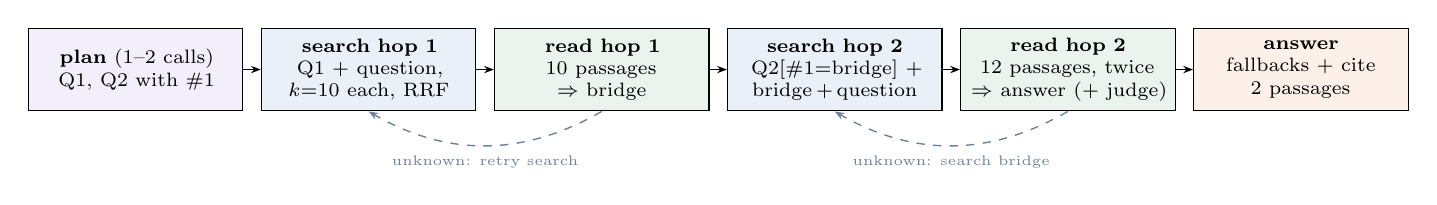
\begin{tikzpicture}[font=\scriptsize, node distance=0.22cm,
  st/.style={draw=black, line width=0.4pt, align=center, text width=2.55cm, inner sep=2.5pt, minimum height=1.05cm},
  arr/.style={-{Stealth[length=3.5pt]}, black, line width=0.5pt}]
  \node[st, fill=cD!10] (p) {\textbf{plan} (1--2 calls)\\Q1, Q2 with \#1};
  \node[st, fill=cA!10, right=of p] (s1) {\textbf{search hop 1}\\Q1 + question, $k{=}10$ each, RRF};
  \node[st, fill=cC!10, right=of s1] (r1) {\textbf{read hop 1}\\10 passages\\$\Rightarrow$ bridge};
  \node[st, fill=cA!10, right=of r1] (s2) {\textbf{search hop 2}\\Q2[\#1=bridge] + bridge\,+\,question};
  \node[st, fill=cC!10, right=of s2] (r2) {\textbf{read hop 2}\\12 passages, twice\\$\Rightarrow$ answer (+ judge)};
  \node[st, fill=cB!10, right=of r2] (a) {\textbf{answer}\\fallbacks + cite 2 passages};
  \foreach \u/\v in {p/s1,s1/r1,r1/s2,s2/r2,r2/a} \draw[arr] (\u) -- (\v);
  \draw[arr, dashed, cG] (r1.south) to[out=-150,in=-30] node[below, font=\tiny]{unknown: retry search} (s1.south);
  \draw[arr, dashed, cG] (r2.south) to[out=-150,in=-30] node[below, font=\tiny]{unknown: search bridge} (s2.south);
\end{tikzpicture}
\end{center}

% =====================================================================
\section{Single-shot vs.\ iterative}
\begin{minipage}[t]{0.585\textwidth}
\vspace{0pt}
\centering\footnotesize
\begin{tabular}{@{}lcccccc@{}}
\toprule
Dev set, 300 questions & EM & Ans.\ F1 & Ev.\ F1 & $S$ & Search & LLM\\
\midrule
B1 single-shot (starter) & 0.1400 & 0.2110 & 0.3717 & 0.2431 & 1.00 & 1.00\\
B2 staff iterative (leaderboard) & 0.2033 & 0.2596 & 0.4767 & 0.3030 & 2.03 & 3.03\\
\textbf{My agent (final)} & \textbf{0.4967} & \textbf{0.5965} & \textbf{0.6650} & \textbf{0.6102} & 4.37 & 5.25\\
\bottomrule
\end{tabular}
\captionof{table}{$S = 0.8\cdot$Ans.\ F1$\,+\,0.2\cdot$Ev.\ F1. Search/LLM = mean calls per question. All 300 ran \texttt{ok}, each far below the 60\,s limit.}
\label{tab:main}
\end{minipage}\hfill
\begin{minipage}[t]{0.395\textwidth}
\vspace{0pt}
\centering\footnotesize
\begin{tabular}{@{}lcc@{}}
\toprule
Diagnostic & B1 & Mine\\
\midrule
both gold paragraphs retrieved & 15.3\% & 69.7\%\\
hop-2 paragraph retrieved & 23.3\% & 72.3\%\\
bridge (hop-1 answer) correct & -- & 76.3\%\\
gold paragraphs cited (of 2) & 0.74 & 1.33\\
\bottomrule
\end{tabular}
\captionof{table}{Why iterating helps (\texttt{dev/analyze.py}).}
\end{minipage}


% =====================================================================
\section{Design}
\textbf{The plan.} A bad split hurts most: answer F1 is 0.48 on the 8 questions left with no split, vs.\
0.60 with one. The plan is re-asked when Q2 lacks \#1, Q1 repeats $\ge$90\% of the question's content words, adds
a kind of place (\emph{birthplace of X}$\to$\emph{which country}), asks \emph{when}/\emph{how many} (a bridge is an
entity, not a date), drops every name the question gives or only asks \emph{who is X}, or copies a prompt example.
The retry prompt names the hidden entity first (five invented examples). If both fail, an
\emph{X's team} or \emph{the Y of X} phrase is split off without the LLM.

\textbf{\texttt{next\_query}.} Each hop sends two $k{=}10$ queries: Q1 and the question at hop~1; Q2 with the
bridge filled in, and bridge + question, at hop~2, without question words (noise for BM25). Reciprocal rank
fusion, $\sum 1/(3+\mathrm{rank})$, puts passages both queries like first. Retries depend on what failed: after a
failed hop-2 read, the bridge alone (its own article), or for \emph{when} questions, whose dates that article
rarely holds, the bridge plus the first sentence of an LLM-written guess passage (Query2doc); after a failed hop-1
read, Q1 plus such a sentence; else the best unsearched passage title plus keywords.

\textbf{Reading.} The LLM sees 10 passages at hop~1 and 12 at hop~2, whole: none exceeds 2,000 characters,
and 5 of 294 answers sit after character 1,200 of their passage. A prompt rejected as too long is retried shorter. Order matters to a 4B model (first hop-1 read: bridge right 83\% with the gold passage first, 71\%
second, 67\% lower), so at hop~1 the article the question names goes first. Only the last read must guess. A bridge read from a passage that is neither first nor that article (47\% right) is re-read after a
Query2doc search. If hop~1 keeps failing, the bridge comes from memory; hop~2 still searches and reads.

\textbf{Checking the hop-2 answer.} A second read uses the same passages reversed and the original question
instead of Q2, which the plan sometimes words badly. If the answers disagree, one call shows both with their passages and asks \emph{``A or B?''}; A, the first, wins any doubt. If the cited
passage lacks the answer but another has it, the evidence is likely mixed up: a second opinion that only repeats
it sends hop~2 back to search. With calls to spare the model also answers Q2 from memory, and the judge decides
again if a passage (retrieved or from a spare search) holds that answer.

\textbf{\texttt{should\_stop}.} Stop once hop~2 has an answer that is not \emph{unknown}, not the bridge and of
the asked type (a date for \emph{when}), or when one LLM call (kept for \texttt{answer}) or under 15\,s is left.
If the server fails a call (after the client's retries), the agent goes on: a failed plan call tries the other
prompt, a failed read counts as failed. With 5\% of calls failing $S$ is 0.601, not 0.539 (15\%: 0.563 vs.\ 0.426).

\textbf{\texttt{answer} and citations.} If hop~2 never answered: a best guess from memory with the bridge as a
hint, then a rejected hop-2 answer of the right type, then a typed span from the best passage. The answer is returned as the model wrote it (only stray markup such as
\emph{Answer:} or quotes is removed). Two citations, chosen after all searches: a passage with the
bridge (preferably the article the question names) and one with the answer (preferably naming the bridge).

\begin{minipage}[t]{0.54\textwidth}
\vspace{0pt}
\centering\footnotesize
\begin{tabular}{@{}lrccc@{}}
\toprule
Plan path or check & $n$ & changed & better/worse & effect\\
\midrule
first plan prompt & 239 & & & F1 0.63\\
second plan prompt & 47 & & & F1 0.47\\
grammar split (no LLM) & 6 & & & F1 0.44\\
no split & 8 & & & F1 0.48\\
\midrule
weak-bridge recheck & 32 & 10 bridges & 3 / 2 & --\\
second read + judge & 178 & 16 & 7 / 0 & $+$0.016 $S$\\
evidence mix-up check & 19 & 3 & 1 / 0 & $+$0.000 $S$\\
memory check + judge & 134 & 5 & 2 / 1 & $+$0.003 $S$\\
\midrule
bridge from memory & 7 & & & F1 0.38\\
memory guess (no hop-2 answer) & 33 & & & F1 0.30\\
\bottomrule
\end{tabular}
\captionof{table}{What each step did in the final dev run. $n$: questions on that path, or where the check made an LLM
call; changed: answers (bridges) it replaced; better/worse against gold; effect: answer F1 of the path, or the change in
$S$ from the replaced answers.}
\label{tab:steps}
\end{minipage}\hfill
\begin{minipage}[t]{0.43\textwidth}
\vspace{0pt}
\textbf{What did not help.} On late versions of this agent: asking for the answer copied word for word
($S$ $-$0.049); a third hop-2 search up front ($-$0.022: retries lose their search); \emph{bridge + rest of Q2} as
the hop-2 retry search, or a second read for answers found on a retry (no gain); shortening answers (extra words cost
only 0.009 of $S$, about as much as missing words). Earlier: quoting the evidence first, a reasoning line, judging
the bridge, backtracking to a new bridge, 14 passages at hop~2, Query2doc for every question (it used the calls the
judge needed). With six calls, checking an answer paid off more than finding more passages.
\end{minipage}

% =====================================================================
\section{Error analysis}
The final agent gets EM $=0$ on 151 of the 300 dev questions. \texttt{dev/analyze.py} labels them automatically:
(i)~35, (ii)~15, (iii)~42, (iv)~51, (v)~8. Many (iv) cases still earn partial credit (\emph{August 5, 1940} vs.\
\emph{5 August 1940} has F1 1.0, EM 0). I labelled 10 of them by hand from their traces (Table~\ref{tab:err}); only
Berthelot disagrees with the automatic label, which says (iii) because both gold paragraphs were retrieved.

\begin{minipage}[t]{0.47\textwidth}
\vspace{0pt}
\centering\footnotesize
\begin{tabular}{@{}lcc@{}}
\toprule
Errors (EM $=0$), auto labels & B1 & final\\
\midrule
(i) bridge entity not found & 191 & 35\\
(ii) stopped too early & 0 & 15\\
(iii) evidence retrieved, wrong answer & 15 & 42\\
(iv) correct but marked wrong & 52 & 51\\
(v) other & 0 & 8\\
\midrule
total & 258 & 151\\
\bottomrule
\end{tabular}
\captionof{table}{Error categories on all 300 dev questions: the single-shot baseline B1 and the final agent.}
\label{tab:cats}
\end{minipage}\hfill
\begin{minipage}[t]{0.505\textwidth}
\vspace{0pt}
\textbf{The bottleneck moved from retrieval to reading.} Iterating cut bridge failures (i) from 191 to 35.
Category (iii) grew from 15 to 42 for the same reason: 209 questions now reach the final read with both gold
paragraphs retrieved (46 for B1), and on those the 4B reader scores answer F1 0.74 (B1: 0.54). The plan checks
and passage ordering target (i); the second read and memory check target (iii): in the final run they replaced
21 answers, 9 for the better and 1 for the worse (Table~\ref{tab:steps}). Reading errors are still the largest class.
\end{minipage}

\begin{center}
\footnotesize\renewcommand{\arraystretch}{1.12}
\begin{tabularx}{\textwidth}{@{}c>{\raggedright\arraybackslash}Xp{2.3cm}p{2.6cm}p{3.9cm}@{}}
\toprule
& Question (shortened) & Gold & Mine & What went wrong\\
\midrule
(i) & Last time Auburn won in the work location of Johnny Berthelot? & 1999 & 1994 & bridge \emph{Gonzales} (hometown), not \emph{Baton Rouge}\\
(i) & Sibling of the composer of \emph{Downtown}? & Astrid Young & Michael Gore & bridge \emph{Luke Laird}, writer of Lady Antebellum's \emph{Downtown}, not Neil Young\\
(i) & When did the civil war start in the country Ita Ford is from? & October 15, 1979 & April 1861 & bridge \emph{United States} (her nationality), not El Salvador\\
(ii) & Manager when Tommy Logan's team won the Champions League? & Roberto Di Matteo & Jos\'e Mourinho & bridge Chelsea right; stopped with a search left, hop-2 paragraph never retrieved\\
(ii) & When did Harrysong's country become a member of OPEC? & 1971 & the 1970s & bridge Nigeria right; vague answer accepted, OPEC table never retrieved\\
(iii) & Where did the 2007 World Series winner get Brandon Phillips from? & Los Angeles Angels & Cleveland Indians & both gold paragraphs retrieved, wrong team read\\
(iii) & Average household size in the city served by WAJM? & 2.46 & 2.50 & second read found 2.46; the judge kept 2.50\\
(iv) & When did the country of Saldus Municipality join the Soviet Union? & 5 August 1940 & August 5, 1940 & same date, other order (F1 1.0, EM 0)\\
(iv) & Forest by the southern border of Jerzy Passendorfer's death city? & Kabaty & Kabaty Forest & correct despite a wrong bridge (\emph{Skolim\'ow}); extra word (F1 0.67)\\
(v) & Who was targeted for defrauding the electoral process, in Hotel Courtland's state? & a whole sentence & John Kerry & gold answer is a sentence; hop-2 paragraph never retrieved\\
\bottomrule
\end{tabularx}
\captionof{table}{Ten hand-labelled errors of the final agent: (i) bridge not found 3, (ii) stopped too early 2, (iii) evidence
retrieved but answered wrongly 2, (iv) correct but marked wrong 2, (v) other 1.}
\label{tab:err}
\end{center}

\textbf{Example 1 (i), Johnny Berthelot.} The plan is right and the gold paragraph is ranked first, but it says
he is \emph{a member of the Louisiana House of Representatives \dots\ based in his hometown of Gonzales}. The model
returns the explicit city; the intended bridge, Baton Rouge (the seat of the legislature), is only implied. Hop~2
asks about Auburn's wins \emph{at Gonzales}: the first read says \emph{unknown}, and the best-guess read takes
\emph{1994} from the gold Auburn--LSU table, which was retrieved, but 1994 is a win \emph{at Auburn, AL}; the last
win at Baton Rouge is 1999. One wrong word at hop~1 decides the question: with a wrong bridge and no hop-2 paragraph answer F1 is
0.14 ($n{=}42$), against 0.76 ($n{=}188$) with the right bridge and the paragraph found.

\textbf{Example 2 (iii), WAJM.} Bridge (\emph{Atlantic City}) and both gold paragraphs are found. Two
near-identical, undated census paragraphs of that article give 2.50 and 2.46 (gold). The first read answers 2.50,
the second read (reversed passages, original question) 2.46, and the judge keeps A (2.50). Because A wins any
doubt, the higher-ranked of two equally plausible passages wins; no passage says which census is meant.

% =====================================================================
\section{AI-use disclosure and code provenance}
I used Claude Code (Anthropic, Claude Opus 5.5) to read the starter code, write the agent and the analysis
scripts in \texttt{dev/}, run the experiments and draft this report. I decided what to try and what to keep,
checked the numbers, and am responsible for the submission. No external code was copied. The loop follows IRCoT
(Trivedi et al., ACL 2023) and ReAct (Yao et al., ICLR 2023); reciprocal rank fusion follows Cormack, Clarke and
Buettcher (SIGIR 2009); the data is MuSiQue (Trivedi et al., TACL 2022). BM25, the tools and the scorer are the
course's \texttt{a4} package. The few-shot examples were written by hand from generic relation types (performer, author,
director, location, employer) and contain no answers. The agent stores no answers or data, never recognises a
question, and returns each answer as the model wrote it.

\end{document}
